\clearpage
%%=========================================
\section{MCT Film Grown by LPE on Substrate B2}\label{sec:subBc}

A film of \ac{mct} was grown on substrate B2 by \ac{lpe}. Nomarski optical microscopy images revealed that the surface of the \ac{mct} film was non-planar in the form of wavy structures with a large number of circular features, as seen in Fig.~\ref{fig:subBc_om}. The same type of circular features were observed on this \ac{mct} film as the one grown on substrate A: Large circular defects with diameter of \SIrange{38}{70}{\micro\metre} and doughnut-shaped defects with diameter of \SIrange{8}{16}{\micro\metre}.

\begin{figure}[htbp]
    \centering
    \mySubfigure{0.49\textwidth}{LPE454_nomarski_grid_21_20x.png}[fig:subBc_om_centre][angle=180]
    \hfill
    \mySubfigure{0.49\textwidth}{LPE454_nomarski_grid_06_20x.png}[fig:subBc_om_edge][angle=180]
    \caption[Nomarski phase contrast microscopy images of \ac{mct} film grown by \ac{lpe} on substrate B2.]{Nomarski phase contrast microscopy images of \ac{mct} film grown by \ac{lpe} on (111)B-oriented substrate B2: \subref{fig:subBc_om_centre} Centre; and \subref{fig:subBc_om_edge} upper right corner.}
    \label{fig:subBc_om}
\end{figure}

%%=========================================
%\subsection{Particles}

Like for the \ac{mct} film on substrate A, the large defects on the \ac{mct} film on substrate B2 were infrequent with respect to the doughnut-shaped defects. Only four large defects were observed in the upper right quadrant of the sample. This gave a large circular defect density of \SI{\sim 2}{\centi\metre^{-2}}, which was the same as for film A. The density of doughnut-shaped defects was, on the other hand, found to be between \SIrange{2e+3}{3e+4}{\centi\metre^{-2}}. The average density was \SI{1e+04}{\centi\metre^{-2}}, with a standard deviation of \SI{5e+03}{\centi\metre^{-2}}. The doughnut-shaped defects were more evenly distributed than on film A, as seen in the graphical representation of the density at different locations on the film in Fig.~\ref{fig:LPE454_densityData}. 

\begin{figure}[htbp]
    \centering
    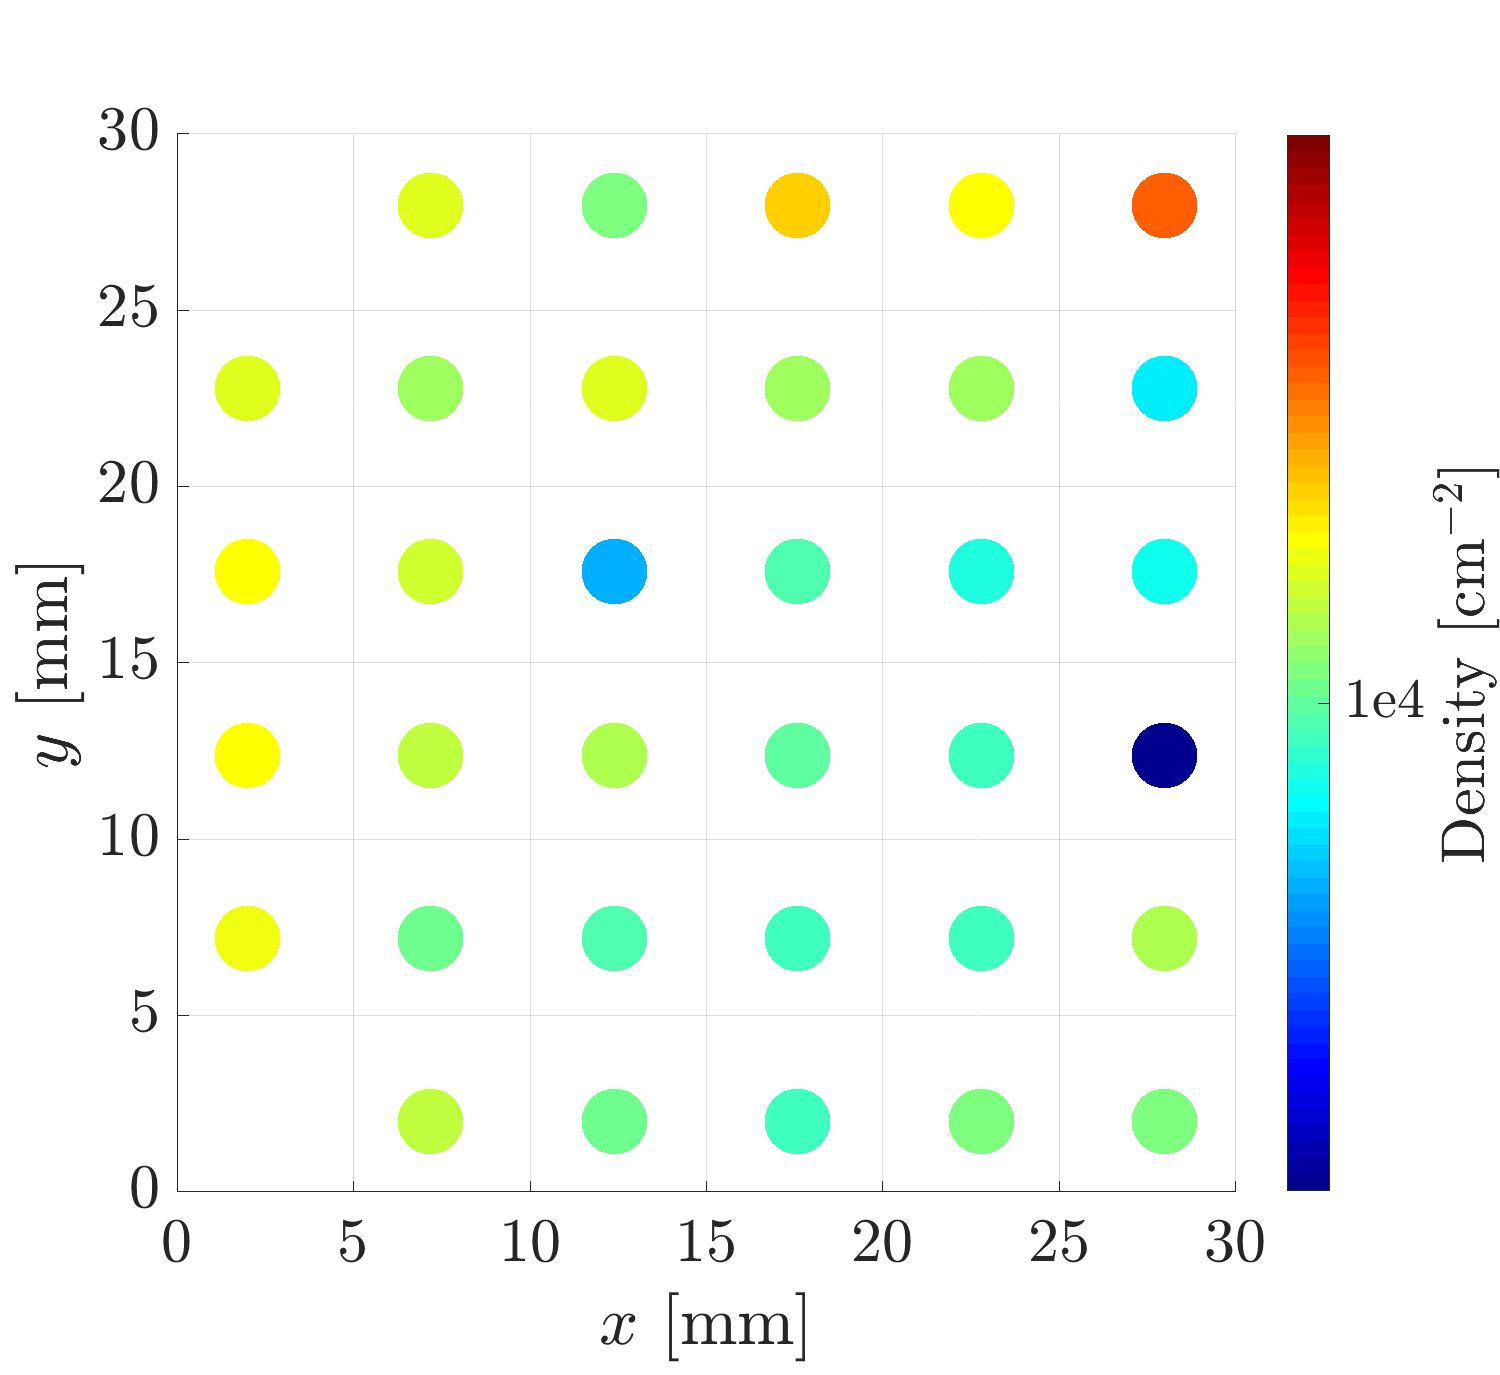
\includegraphics[width=0.5\linewidth]{LPE454_densityData.png}
    \caption[Map of the density of doughnut shaped structures on the \ac{mct} film grown on substrate B2.]{A map of the density of doughnut shaped structures at 34 different locations on the $\SI{30}{\milli\metre}\times\SI{30}{\milli\metre}$ \ac{mct} film grown on substrate B2. The density measurements were obtained by counting the number of doughnut-shaped defects in Nomarski optical microscopy images covering $\SI{558}{\micro\metre}\times\SI{419}{\micro\metre}$ areas. In total, \SI{0.94}{\percent} of the substrate surface was measured. The density was observed to vary between \SIrange{2e+3}{3e+4}{\centi\metre^{-2}} with an average defect density of \SI{1e+04}{\centi\metre^{-2}}.}
    \label{fig:LPE454_densityData}
\end{figure}

The sample Pearson correlation coefficient between the occurrence of polishing grit on substrate B2 and the occurrence of doughnut-shaped defects on the film was determined to be \SI{+0.68}{}, which is a strong positive correlation. As the occurrence of polishing grit on substrate A and the occurrence of doughnut-shaped defects on the corresponding film showed no correlation, this relation should be investigated further in future studies.%\todo{Sammenlign med telling av tellurium precipitates.}

%It was observed an increased number of doughnut-shaped defects inside \ac{sem} contaminated rectangles.

Similarly to the film grown on substrate A, there were found spherical carbon-based particles and boron nitride particles in connection with a few of the doughnut-shaped defects. In addition, \ac{mct} particles was found towards the edges of the film.

%%=========================================
\subsection{Composition and Thickness}

\Ac{ftir} transmission spectra were recorded from the \ac{mct} film at the same $11\times11$ grid spots as before growth. The \ac{ir} transmittance was between \SIrange{0}{42}{\percent} in the wavenumber range between \SIrange{400}{1400}{\centi\metre^{-1}}, see Fig.~\ref{fig:subBc_ftir}. As for the film grown on substrate A, this film must be annealed to reduce the metal vacancy concentration before further fabrication. The average cut-on wavenumber was \SI{2083.3}{\centi\metre^{-1}}, which corresponds to a wavelength of \SI{4.80}{\micro\metre}. Consequently, the $x$-value was \SI{0.269}{} according to the Brice equation \citep{brice1975some}. The thickness of the \ac{mct} film was calculated to be on average \SI{28.1}{\micro\metre} by using Eq.~\ref{eq:ftir_thickness}.

\begin{figure}[htbp]
    \centering
    \mySubfigure{0.60175438596\linewidth}{LPE454_ftir_spectra.png}[fig:subB2c_ftir_spectra]
    \hfill
    \mySubfigure{0.37824561403\linewidth}{LPE454_ftir_transmission_at_k500cm-1.png}[fig:subB2c_ftir_map_500cm-1]
    \caption[\Ac{ftir} measurements of the \ac{mct} film grown on substrate B2.]{\Ac{ftir} measurements recorded from a $11\times11$ grid on the $\SI{30}{\milli\metre}\times\SI{30}{\milli\metre}$ \ac{mct} film grown on substrate B2: \subref{fig:subB2c_ftir_spectra} Transmission spectra; \subref{fig:subB2c_ftir_map_500cm-1} transmission map at wavenumber $k=\SI{500}{\centi\metre^{-1}}$ showing the transmittance $T$ in percentage of incoming light at each grid point.}\label{fig:subBc_ftir}
\end{figure}
%\todo{FTIR: correlate with polishing grit or doughnut density.}

%%=========================================
\subsection{Impurity Analysis -- EDS}

\Ac{eds} was used to get a quantitative analysis of the chemical composition of the \ac{mct} film grown by \ac{lpe} on substrate A. The results can be seen in Table~\ref{tab:subBc_eds_analysis}. The following elements were identified: \ce{Te}, \ce{Hg}, \ce{Cd}, \ce{C}, \ce{O}, and \ce{Al}. The relative concentrations of \ce{Cd}, \ce{Zn}, and \ce{Te} were \ce{Hg_{0.71}Cd_{0.28}Te_{1.01}}, \ce{Hg_{0.74}Cd_{0.25}Te_{1.01}}, and \ce{Hg_{0.74}Cd_{0.25}Te_{1.01}} for the centre, edge, and corner respectively. 

\begin{table}[htbp]
    \centering
    \caption[\Ac{eds} impurity analysis of \ac{mct} film grown by \ac{lpe} on substrate A.]{Results of the \ac{eds} impurity analysis at three different locations on the $\SI{30}{\milli\metre}\times\SI{30}{\milli\metre}$ \ac{mct} film grown by \ac{lpe} on (111)B-oriented substrate A (atomic concentration \%). The X-ray signal was acquired from $\SI{1270}{\micro\metre}\times\SI{890}{\micro\metre}$ areas near the centre, upper edge, and upper left corner.}\label{tab:subBc_eds_analysis}
   \begin{tabu} to 1.0\textwidth { X[1.85, r] X[1.125,c] X[1.125,c] X[1.125,c] X[1.125,c] X[1.125,c] X[1.125,c] }
        \hline
            & \textbf{\ce{Te}} (at.\%) & \textbf{\ce{Hg}} (at.\%) & \textbf{\ce{Cd}} (at.\%) & \textbf{\ce{C} } (at.\%) & \textbf{\,\ce{O}\,} (at.\%) & \textbf{\ce{Al}} (at.\%) \\
        \hline
        Near centre & \SI{44,36}{} & \SI{31,14}{} & \SI{12,19}{} & \SI{11,30}{} & \SI{0,86}{} & \SI{0,16}{} \\
        Near edge & \SI{44,12}{} & \SI{32,26}{} & \SI{10,81}{} & \SI{11,49}{} & \SI{1,14}{} & \SI{0,18}{} \\
        Near corner & \SI{44,26}{} & \SI{32,58}{} & \SI{10,71}{} & \SI{11,23}{} & \SI{1,03}{} & \SI{0,19}{}  \\
        \hline
    \end{tabu}
\end{table}


%%=========================================


\begin{comment}
\section{LPE - Hall, FTIR, SIMS}

\todo{Have to add SIMS to both Method chapter and Experimental details chapter (Why is SIMS used?).} \Ac{sims} profiles of \ce{Na}, \ce{Al}, \ce{Si}, \ce{K}, \ce{Fe}, \ce{Ni}, \ce{Cu}, and \ce{Pb} from two different locations on sample LPE422 are shown in Fig.~\ref{fig:sims_lpe422}. The measurements show that \ce{Na}, \ce{Al}, \ce{Si}, \ce{K}, and \ce{Fe} are found at the interface between the substrate and the grown layer as peak concentrations. \ce{Ni}, \ce{Cu}, and \ce{Pb}, with detection limits of \SI{1e14}{}, \SI{2e14}{}, and \SI{2e13}{\atom\centi\metre^{-3}} respectively, were not detected throughout the \ce{HgCdTe} film and \ce{CdZnTe} substrate.

\ce{Si} and \ce{K} were detected in neither the \ce{HgCdTe} film nor in the \ce{CdZnTe} substrate. \todo{Where does the Si and K come from?}

\ce{Na} and \ce{Al} were not detected in the \ce{HgCdTe} film, but were detected in the \ce{CdZnTe} substrate. \todo{Why doesn't Al diffuse into the layer? Why is there a minimum in the Na concentration right after the peak before it grows into the substrate?}

\ce{Fe} was detected throughout both the \ce{HgCdTe} layer and the \ce{CdZnTe} substrate. Higher \ce{Fe} concentration was detected with a peak \ce{Fe} concentration likely at the interface of \ce{HgCdTe} and \ce{CdZnTe}. This higher concentration of \ce{Fe} was found between a depth of \SI{\sim 13}{\micro\metre} and \SI{23}{\micro\metre} for the first measurement, and between a depth of \SI{\sim 16}{\micro\metre} and \SI{23}{\micro\metre} for the second measurement. The \ce{Fe} peak stands out \todo{... explanation of the different shapes: Why does the \ce{Fe} concentration have a wide concentration peak? And why is it in both the substrate and the layer?} \todo{Group 1A and 1B diffuse faster than other?}

%\todo{Cadmium is cation, and tellurium is anion.}

\todo{\Ac{ftir}}

\todo{Hall}

\begin{figure}[htbp]
    \centering
    \subfigure[W3]{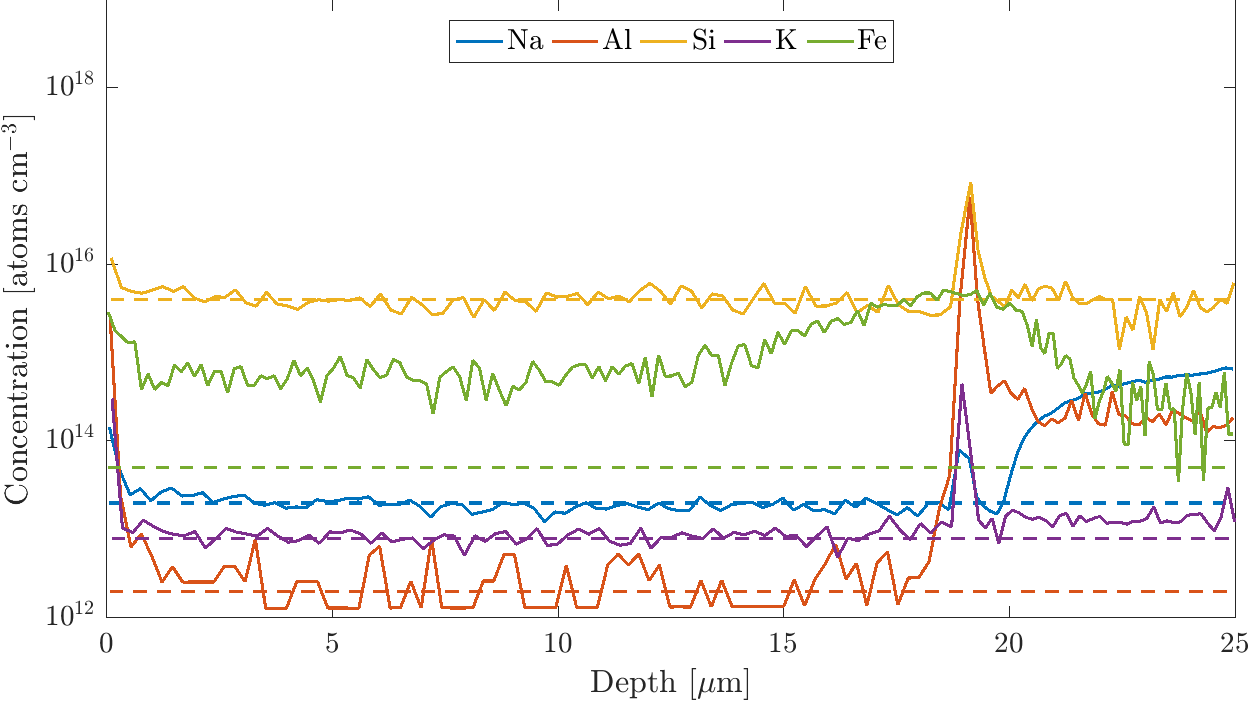
\includegraphics[width=0.90\linewidth]{sims_lpe422_w3.png}}
    %\quad
    \subfigure[W4]{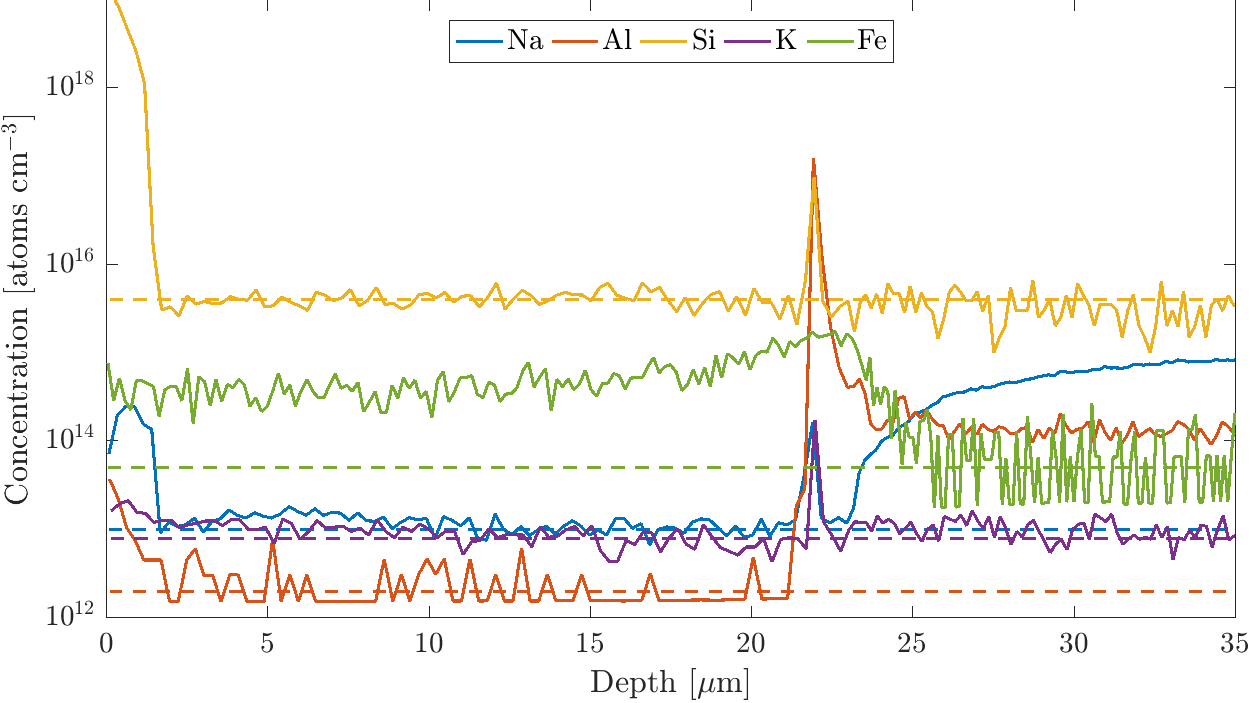
\includegraphics[width=0.90\linewidth]{sims_lpe422_w4.png}}
    \caption[\Ac{sims} profiles from sample LPE422.]{\Ac{sims} profiles of \ce{Na}, \ce{Al}, \ce{Si}, \ce{K}, and \ce{Fe} atom concentration in sample LPE422. These are the profiles for the epitaxial \ce{HgCdTe} layer grown by \ac{lpe} on a (111)B \ce{CdZnTe} substrate from vendor B. \ce{Ni}, \ce{Cu}, and \ce{Pb}, with detection limits of \SI{1e14}{}, \SI{2e14}{}, and \SI{2e13}{\atom\centi\metre^{-3}} respectively, were not detected. The solid line is the concentration of an element, while the dashed line is the detection limit of that element.}
    \label{fig:sims_lpe422}
\end{figure}
%%=========================================

\todo{LPE smelte størkner tidligere ved urenheter -> krystallinske defekter i laget.}
\end{comment}